% !Mode:: "TeX:UTF-8:Main"
%improves compability with tikz etc ...
\PassOptionsToPackage{patches}{pdfresources}

\documentclass{article}
\usepackage{pdfpages,xcolor}

% use a custom hyperref driver:
\usepackage[customdriver=hgeneric-experimental]{hyperref}
\hypersetup{linkbordercolor=blue}
\hypupdateattribute %after \hypersetup

\usepackage{newpax}

%use the link border color and style of the imported pdf
%and not hyperref colors
\newpaxsetup{usefileattributes=true}

\begin{document}

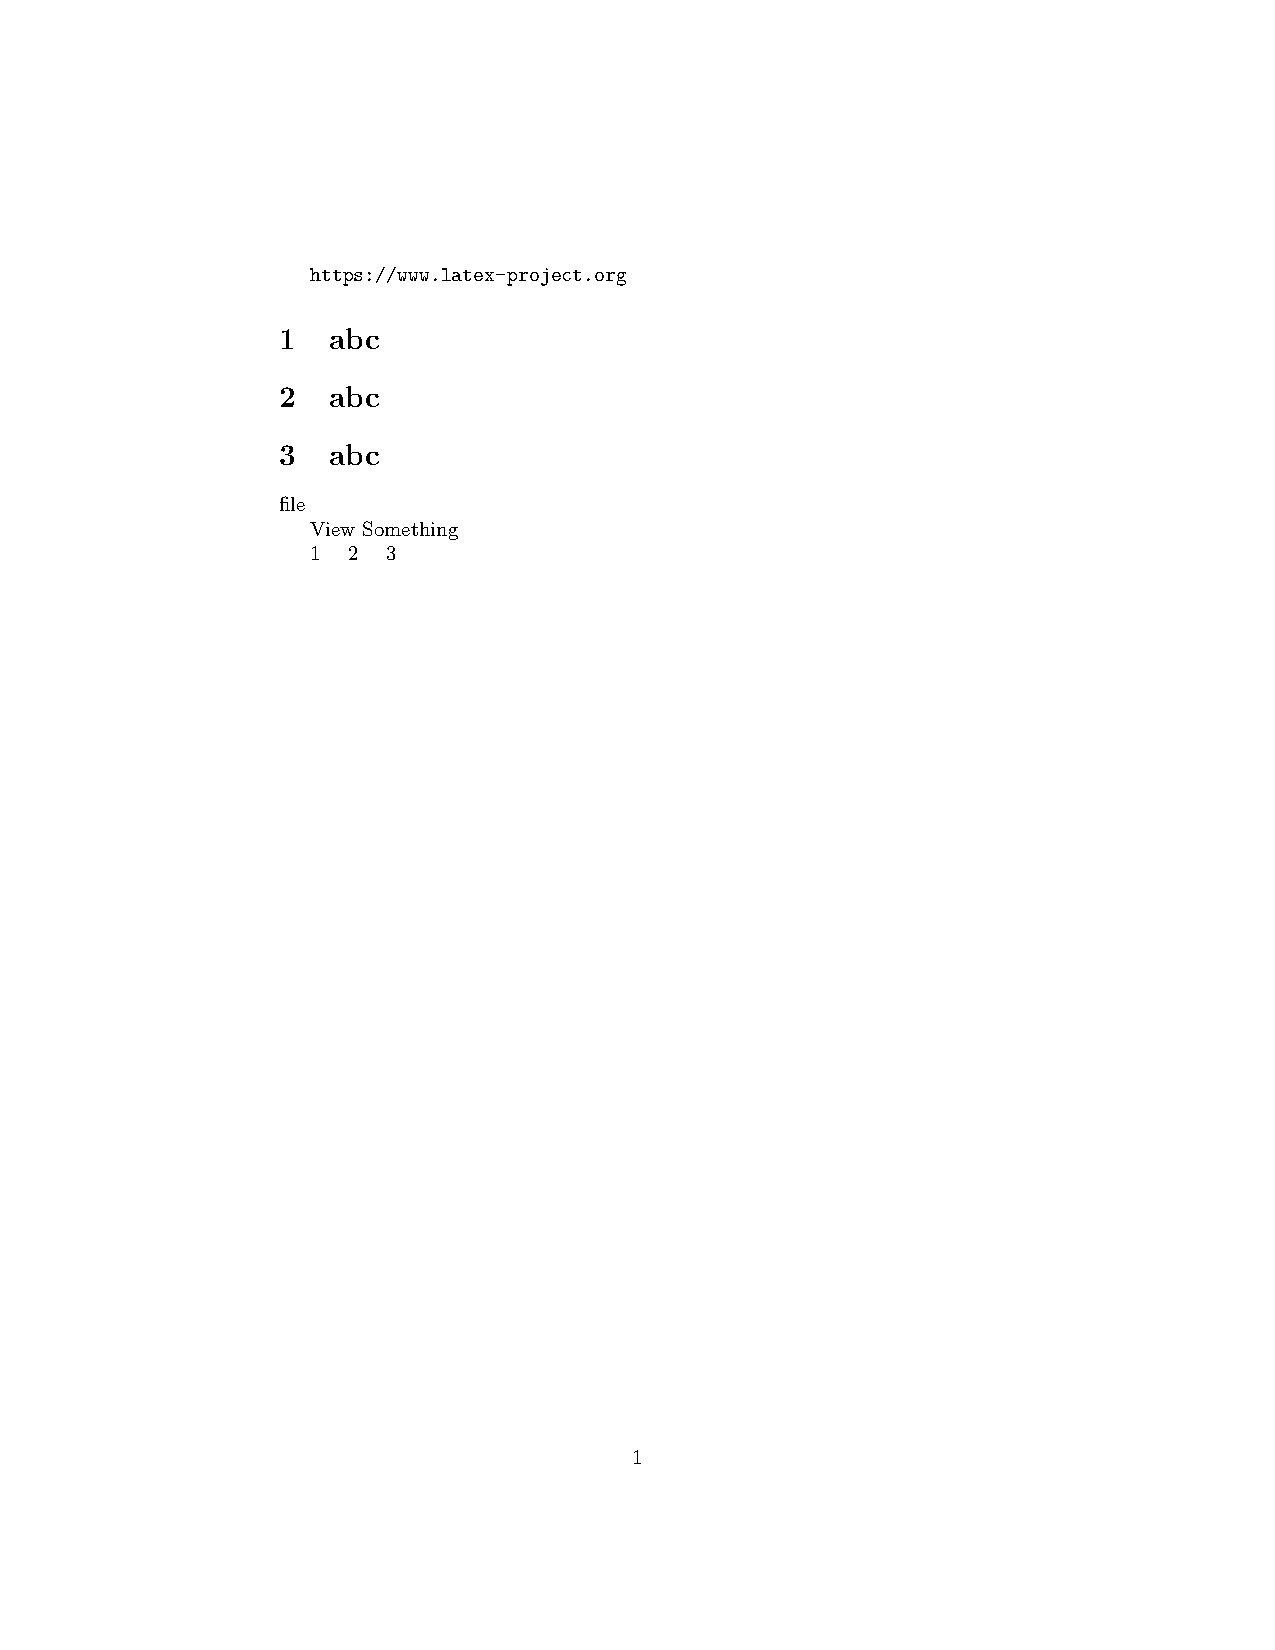
\includegraphics[scale=0.5,trim=4cm 15cm 8cm 3cm,clip,page=1]{pax-input}
\includegraphics[scale=0.5,trim=5cm 15cm 8cm 3cm,clip,page=2]{pax-input}

%set a unique suffix is the pdf is imported twice
\newpaxsetup{destsuffix=B} 
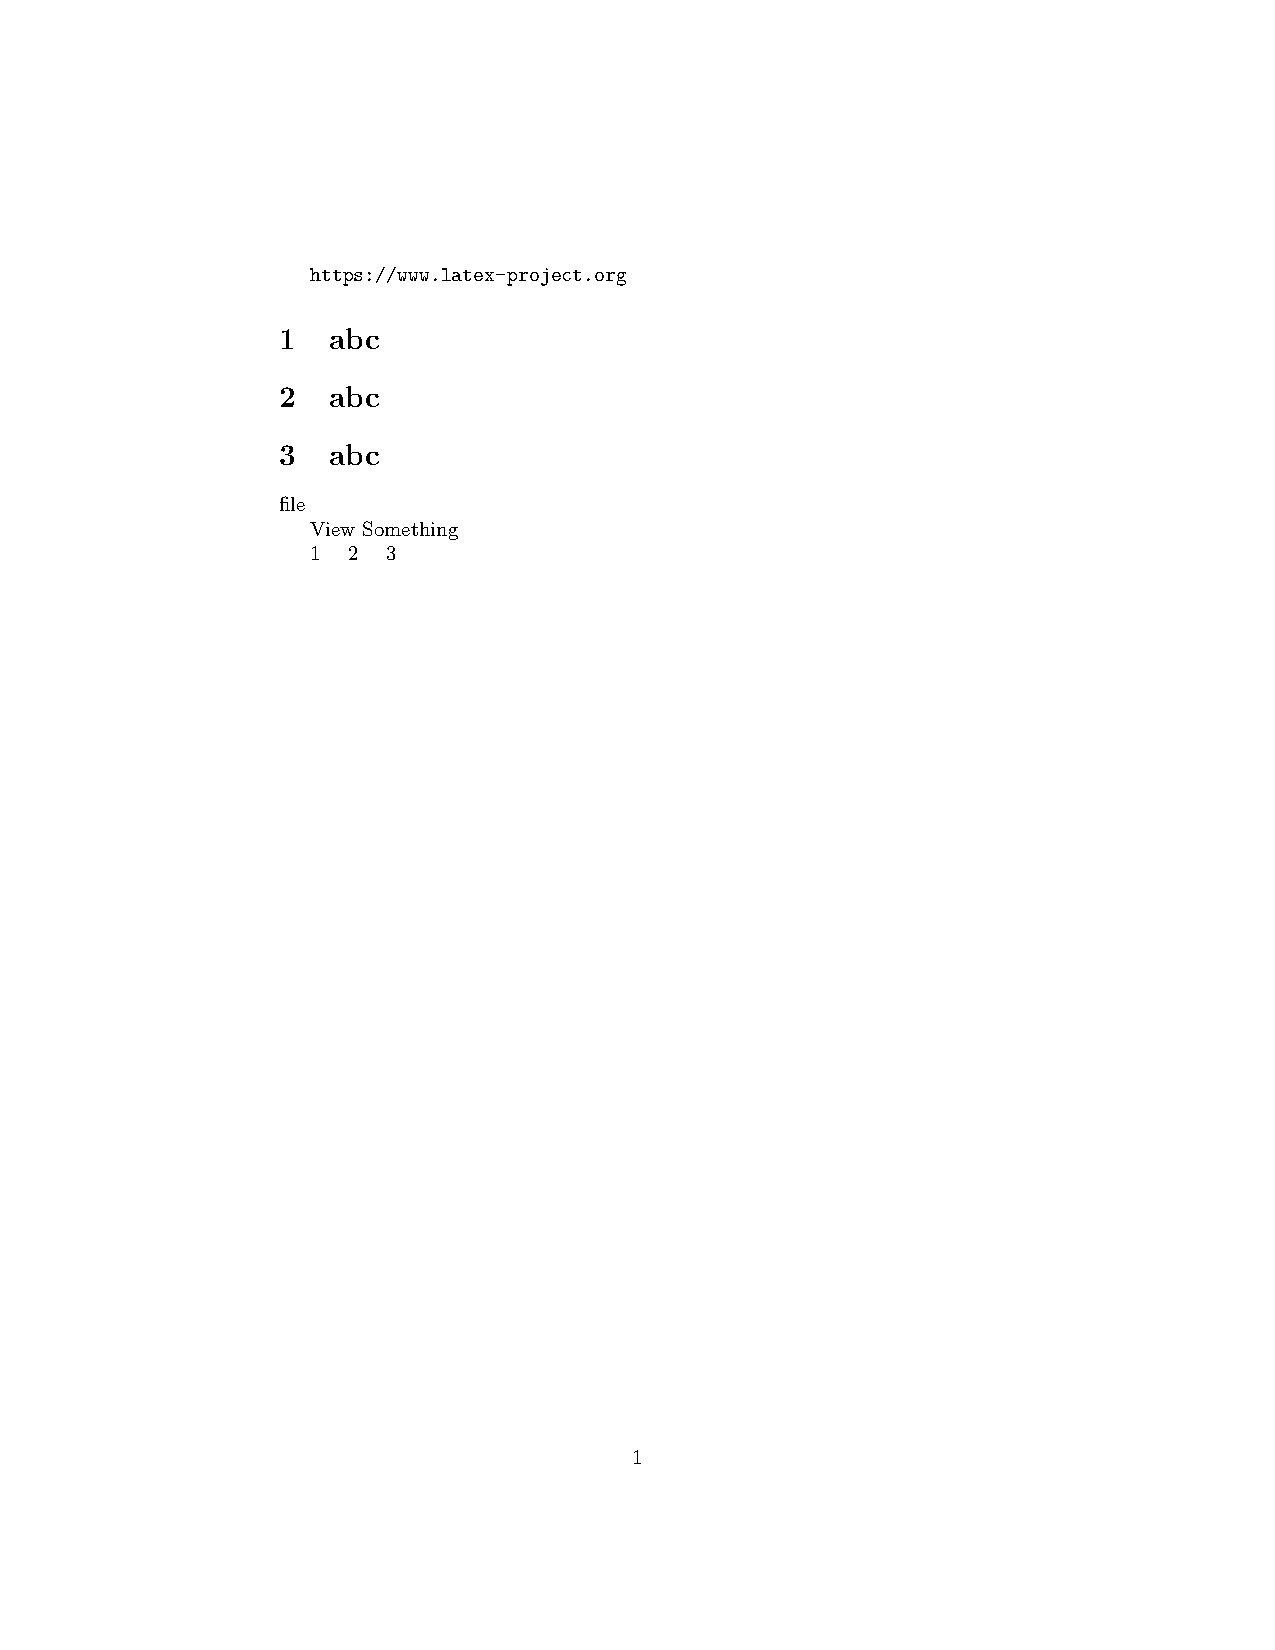
\includegraphics[scale=0.5,trim=4cm 15cm 8cm 3cm,clip,page=1]{pax-input}
\includegraphics[scale=0.5,trim=5cm 15cm 8cm 3cm,clip,page=2]{pax-input}

% suppress the adding of annotations
\newpaxsetup{addannots=false}
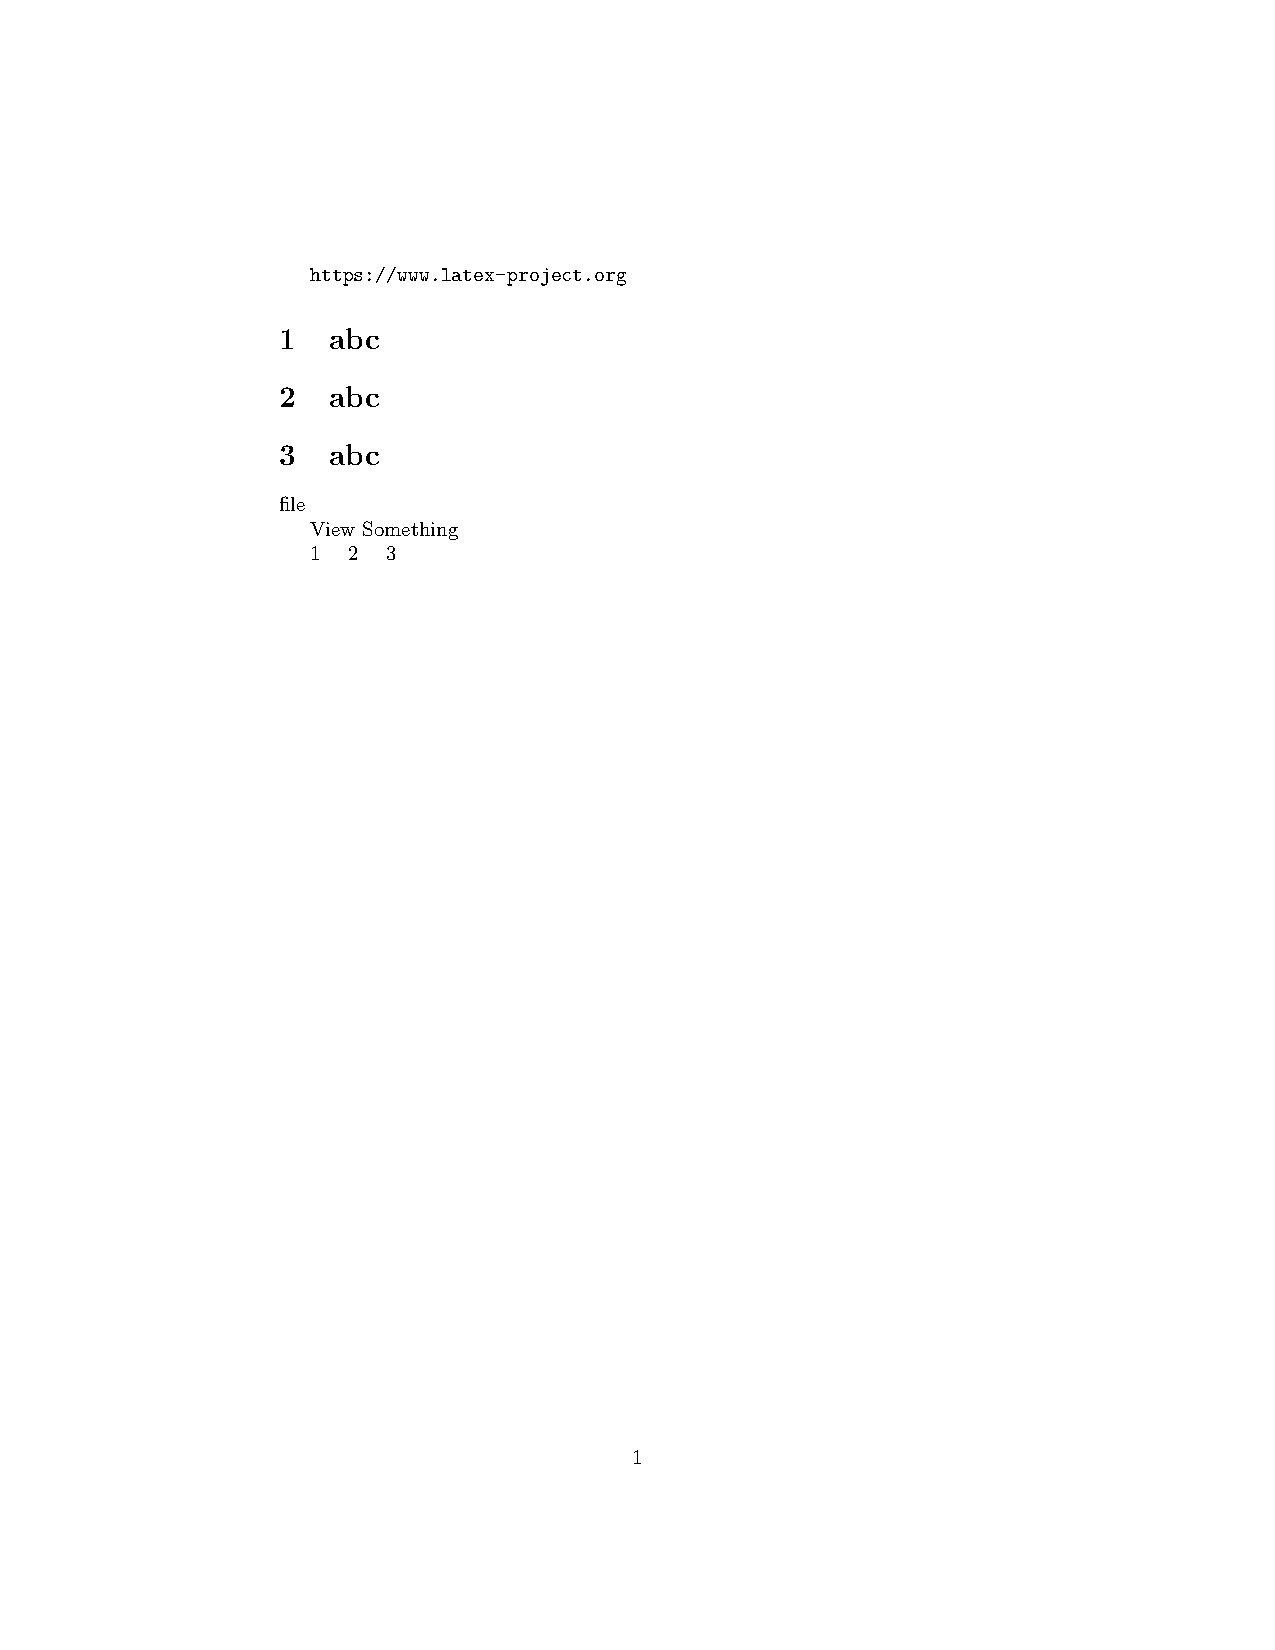
\includegraphics[scale=0.5,trim=4cm 15cm 8cm 3cm,clip,page=1]{pax-input}

%reactivate
\newpaxsetup{addannots=true}
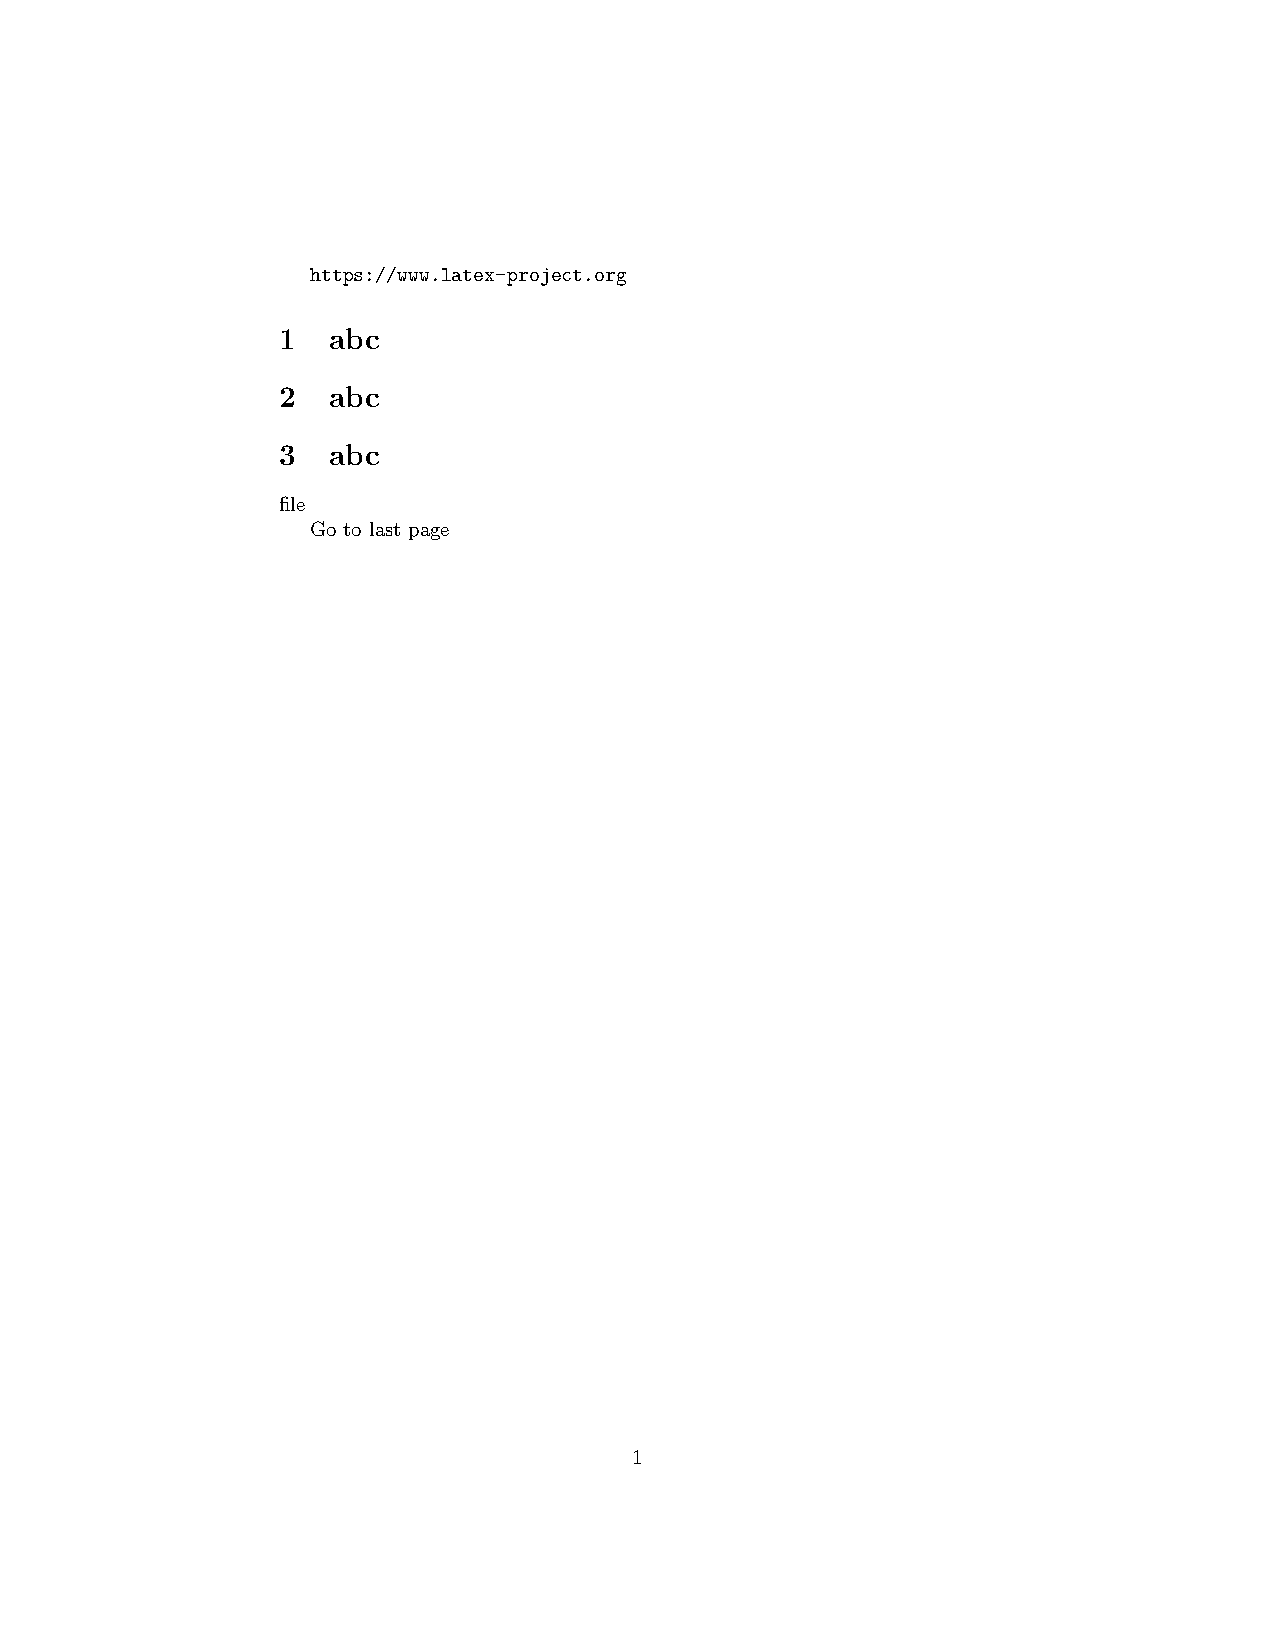
\includepdf[pages=-]{figure/pax-input2}
\end{document}
